\documentclass[12pt, twoside]{article}
\usepackage[letterpaper, margin=1in, headsep=0.2in]{geometry}
\setlength{\headheight}{0.6in}
%\usepackage[english]{babel}
\usepackage[utf8]{inputenc}
\usepackage{microtype}
\usepackage{amsmath}
\usepackage{amssymb}
%\usepackage{amsfonts}
\usepackage{siunitx} %units in math. eg 20\milli\meter
\usepackage{yhmath} % for arcs, overparenth command
\usepackage{tikz} %graphics
\usetikzlibrary{quotes, angles}
\usepackage{graphicx} %consider setting \graphicspath{{images/}}
\usepackage{parskip} %no paragraph indent
\usepackage{enumitem}
\usepackage{multicol}
\usepackage{venndiagram}

\usepackage{fancyhdr}
\pagestyle{fancy}
\fancyhf{}
\renewcommand{\headrulewidth}{0pt} % disable the underline of the header
\raggedbottom
\hfuzz=2mm %suppresses overfull box warnings

\usepackage{hyperref}

\fancyhead[LE]{\thepage}
\fancyhead[RO]{\thepage \\ Name: \hspace{4cm} \,\\}
\fancyhead[LO]{BECA / Dr. Huson / Geometry\\*  Unit 3: Parallel lines and transversals\\* 20 October 2022}

\begin{document}

\subsubsection*{3.3 Homework: Mixed review}
\begin{enumerate}
\item Apply the Angle Addition postulate. Write and equation to support your work.
  \begin{multicols}{2}
    Given m$\angle ABD = 75^\circ$, m$\angle ABC = 90^\circ$. \par \bigskip
    Find $m \angle CBD$. \par
    \begin{tikzpicture}[scale=1.4]
      \draw[<->, thick]
        (0:3) coordinate (a) node[below left] {$C$}
        -- (0,0) coordinate (b) node[below left] {$B$}
        -- (20:3) coordinate (c) node[below right] {$D$}
        pic["$?$", <->, draw=black, angle eccentricity=1.5, angle radius=1cm]
        {angle=a--b--c};
        \draw[<-, thick]
        (90:2) coordinate (d) node[right] {$A$}
        -- (0,0) coordinate (e)
        pic["$75$", <->, draw=black, angle eccentricity=1.5, angle radius=1cm]
        {angle=c--e--d};
      \draw (0,0)++(0.3,0)--++(0,0.3)--+(-0.3,0);
    \end{tikzpicture}
  \end{multicols}

\item Given vertical angles, m$\angle APD = 9x-1$, m$\angle BPC = 6x+20$, as shown. \par \medskip
  Find $x$. Check your solution for full credit.
  \begin{flushright}
    \begin{tikzpicture}[scale=1.6, rotate=-35]
      \draw[<->, thick] 
        (0:-2)node[above right]{$A$}--
        (0:2)node[below left]{$C$};
      \draw[<->, thick] 
        (60:-2)node[above left] {$D$}--node[below]{$P$}
        (60:2)node[below right]{$B$};
      \node at (30:1.2){$6x+20$};
      \node at (30:-1.2){$9x-1$};
    \end{tikzpicture} 
    \end{flushright} \vspace{1cm}

\item Ray $\overrightarrow{BF}$ is the angle bisector of $\angle ABC$. Given that the angle measures are m$\angle ABF = 7x+9$ and m$\angle CBF = 9x-13$. \par \bigskip
  Find m$\angle ABC$. \vspace{0.5cm}
    \begin{flushright}
      \begin{tikzpicture}[scale=1, rotate=40]
        \draw[<->, thick]
          (0:3) coordinate (a) node[above left] {$C$}
          -- (0,0) coordinate (b) node[below] {$B$}
          -- (80:3) coordinate (c) node[above right] {$F$}
          pic["$9x-13$", <->, draw=black, angle eccentricity=1.25, angle radius=1.5cm]
          {angle=a--b--c};
          \draw[<-, thick]
          (160:3) coordinate (d) node[above left] {$A$}
          -- (0,0) coordinate (e)
          pic["$7x+9$", <->, draw=black, angle eccentricity=1.5, angle radius=1.5cm]
          {angle=c--e--d};
      \end{tikzpicture}
    \end{flushright}

\newpage
\item Find $m\angle 1$ given two parallel lines and a transversal, with
  \begin{multicols}{2}
  $\displaystyle m\angle 3 = 2x+17$ \hspace{0.75cm}$\displaystyle m\angle 5 = 4x-5$
  \begin{flushright}
    \begin{tikzpicture}[scale=1,rotate=-10]
      \draw [<->, thick] (3,2)--(8,2);
      \draw [<->, thick] (2,0)--(7,0);
      \draw [<->, thick] (4,-1)--(5.5,3);
      \node at (4.5,0.3) [left]{$5$};
      \node at (4.5,0.3) [right]{$6$};
      \node at (4.3,-0.3) [left]{$7$};
      \node at (4.3,-0.3) [right]{$8$};
      \node at (5.2,2) [above left]{$1$};
      \node at (5.4,2) [above right]{$2$};
      \node at (4.9,2) [below left]{$3$};
      \node at (5,2) [below right]{$4$};
    \end{tikzpicture}
  \end{flushright} 
  \end{multicols} \vspace{2cm}

\item Given $\overleftrightarrow{ABC}$, right angle $\angle DBE$, m$\angle ABE = 4x+12$, and m$\angle CBD = 3x-6$. \par \bigskip
  Find m$\angle CBD$. \vspace{0.5cm}
    \begin{flushright}
      \begin{tikzpicture}[scale=1, rotate=10]
        \draw[<->, thick]
          (-30:3.5) coordinate (a) node[below] {$C$}
          -- (0,0) coordinate (b) node[below] {$B$}
          -- (3,0) coordinate (c) node[above left] {$D$}
          pic["$3x-6$", <->, draw=black, angle eccentricity=1.5, angle radius=1.5cm]
          {angle=a--b--c};
          \draw[<->, thick]
          (150:3) coordinate (d) node[below left] {$A$}
          -- (0,0) -- (0, 3) coordinate (e) node[above right] {$E$}
          pic["$4x+12$", <->, draw=black, angle eccentricity=1.5, angle radius=1.5cm]
          {angle=e--b--d};
          \draw (0,0)++(0.4,0)--++(0,0.4)--+(-0.4,0);
      \end{tikzpicture}
    \end{flushright}
  
\item Ray $\overrightarrow{XL}$ is the angle bisector of $\angle KXM$. Given m$\angle JXN = 2x+3$. \par \bigskip
Find $x$.
  \begin{flushleft}
  \begin{tikzpicture}[scale=1, rotate=0]
    \draw[<->, thick] (-135:2)--(0,0)--(45:3);
    \draw[<->, thick] (-2,0)--(3,0);
    \draw[->, thick] (0,0)--(0,3);
    \draw (0,0)++(-0.3,0)--++(0,0.3)--+(0.3,0);
    \draw[fill] (45:2) circle [radius=0.05] node[right]{$L$};
    \draw[fill] (-1.5,0) circle [radius=0.05] node[above left]{$J$}; 
    \draw[fill] (0,0) circle [radius=0.05] node[below right]{$X$};
    \draw[fill] (0,2) circle [radius=0.05] node[left]{$K$};
    \draw[fill] (2,0) circle [radius=0.05] node[below right]{$M$};
    \draw[fill] (-135:1.5) circle [radius=0.05] node[right]{$N$};
  \end{tikzpicture}
  \end{flushleft}


\end{enumerate}
\end{document}